
%(BEGIN_QUESTION)
% Copyright 2012, Tony R. Kuphaldt, released under the Creative Commons Attribution License (v 1.0)
% This means you may do almost anything with this work of mine, so long as you give me proper credit

Examine this process trend showing the PV, SP, and Output of a loop controller:

$$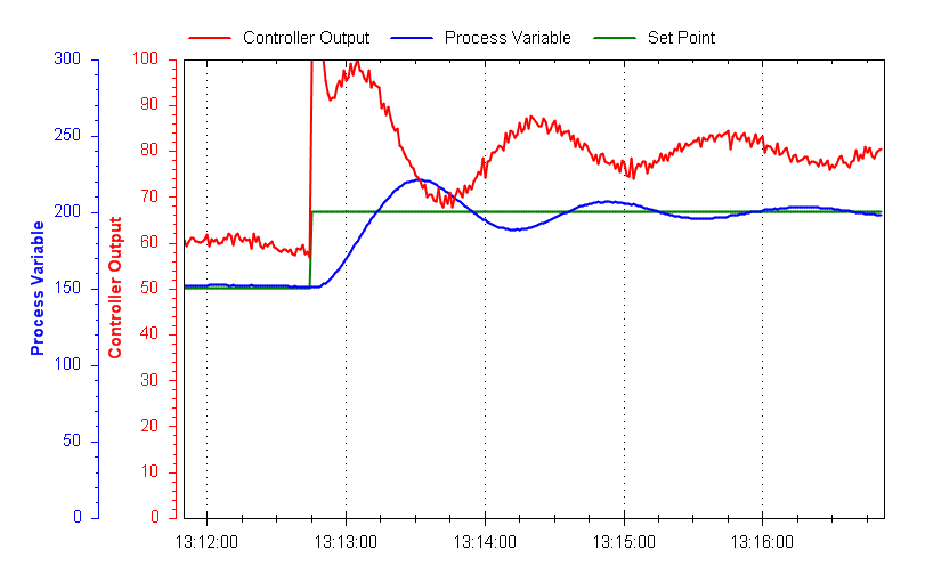
\includegraphics[width=15.5cm]{i01928x01.eps}$$

Based on what you see here, determine the following:

\begin{itemize}
\item{} Whether this is an open-loop or a closed-loop response
\item{} Whether the controller is (or needs to be) {\it direct-acting} or {\it reverse-acting}
\item{} If possible, identify any problems with the field instrumentation
\item{} If possible, identify any problems with the controller PID tuning
\item{} Qualitatively identify the kind of PID tuning we will need for robust control
\end{itemize}

\underbar{file i01928}
%(END_QUESTION)





%(BEGIN_ANSWER)

This is a {\it closed-loop test}, based on the fact the output signal responds dynamically to the changing process variable, as well as to the step-change in setpoint.

\vskip 10pt

This is a {\it reverse-acting} controller: the output steps up when the setpoint steps up (implying the output would step down if the process variable stepped up).

\vskip 10pt

We really cannot discern any problems with field instrumentation from this trend.  A manual-mode (open-loop) test would be more informative in that regard.

\vskip 10pt

The oscillation around setpoint shows that something is tuned too aggressively for the process.  Based on the lagging phase shift of the output waveform, it looks as though integral action is the one that's too aggressive.  It also appears we may have too much derivative action, based on the amount of noise present on the output signal versus the relatively ``quiet'' process variable signal.  It would take a huge amount of gain to make proportional action amplify noise to this extent, and we can see by comparing the output oscillations versus the process variable oscillations that our gain cannot be much greater than 2.

\vskip 10pt

Less derivative action (to tone down the noise amplification on the output), for sure!  Less integral action to avoid the oscillation around setpoint.

%(END_ANSWER)





%(BEGIN_NOTES)


%INDEX% Control, PID tuning: step change (output) revealing poor controller tuning
%INDEX% Process troubleshooting: diagnosing problem via trend recording

%(END_NOTES)


